% !TeX encoding = UTF-8
% !TeX program = xelatex+shellescape+bibtex
% !TeX spellcheck = LaTeX
%
% Author : Shlw
\documentclass[a4paper,12pt]{article}

\usepackage{amsmath}
\usepackage{graphicx}
\usepackage{hyperref}
\usepackage{caption,subcaption}
\usepackage{xcolor}
\usepackage{minted}
\usepackage{ctex}
\usepackage{dingbat}
\usepackage{listings}
\usepackage{geometry}
\usepackage{amssymb}
\usepackage[ruled]{algorithm2e}
\usepackage{ntheorem}
\usepackage{pgfplots}
\usepackage{verbatim}

\hypersetup{hidelinks}
\pgfplotsset{width=8cm}
\geometry{left=3cm,right=3cm,top=3cm,bottom=3cm}
\definecolor{bg}{rgb}{0.95,0.95,0.95}
\renewcommand{\listingscaption}[1]{\begin{center}CODE: #1\end{center}\vspace{-20pt}}
\setminted{
bgcolor=bg,frame=lines,
mathescape,breaklines,breakanywhere,
breaksymbolleft=\raisebox{0.8ex}{\small\reflectbox{\carriagereturn}},
breaksymbolright=\small\carriagereturn
}
\bibliographystyle{plain}
{
\theoremstyle{plain}
\theorembodyfont{\normalfont}
\newtheorem{thmdef}{\hspace{\parindent}定义}
}
\numberwithin{thmdef}{section}

\begin{document}
\begin{titlepage}
    \mbox{}
    \vskip 8 cm
    \centering
    \Huge Progressive Photon Mapping\\ \huge ---计算机图形学大作业报告

    \rule{\textwidth}{1pt}\par % Thick horizontal line

    \Large 吴克文\ 梁家硕

    \large 2017年6月
\end{titlepage}
\tableofcontents
\newpage
\section{综述}
Photon Mapping作为全局光照领域的主流算法,以其高效率,能处理多种光照效果%
等特点,一直受到广泛的关注。\par
然而,Photon Mapping算法的一个主要问题在于,使用光子进行光能估计的过程引入%
了偏差。理论上,要完全消除偏差,需要存储无穷的光子,这从计算机存储角度来看%
是不可接受的。\par
为此,Toshiya Hachisuka提出了Progressive Photon Mapping(又称渐进式%
光子映射),采用多遍的绘制流程,通过不断向场景中发射光子达到不断减小偏差的%
目的,亦解决了Photon Mapping的存储问题。
\section{编译与运行环境}
Linux/Windows (仅在Archlinux与Windows7环境下做过测试)\par
支持c++11的编译器\par
GNU toolchain\par
cmake >= 2.8\par
\begin{minted}{shell}
     $ cd <directory_of_Equestrotopia>
     $ cmake .
     $ make 
\end{minted}

这样会在bin目录下产生raytracing,photontracing,passes,updation四个可执行文件,以及Equestrotopia和lodepng两个动态连接库文件。\par
四个可执行文件的作用可由名称看出,passes是raytracing和photontracing的结合版。\par
使用方法:
\begin{minted}{shell}
    $ photontracing <directory>
    $ updation <directory> <picture_name>
\end{minted}
四个可执行文件的使用方法都是在命令行参数里指定一个目录的名称。\par
该目录下应包含物体列表文件list.txt,光源参数文件light.txt,摄像机参数文件camera.txt,光子贡献比例文件photon\_contrib.txt,以及list.txt中列出的obj格式的文件和球体文件,和obj文件里列出的mtl格式的文件。\par
list.txt文件格式:
\begin{itemize}
    \small \setlength{\itemsep}{.1em}
    \item 第一行,一个整数n,表示接下来obj格式的文件的数目
    \item 接下来n行,每行一个obj格式的文件的文件名
    \item 接下来一行,一个整数m,表示球体文件数目
    \item 接下来m行,每行一个球体文件的文件名
\end{itemize}
light.txt文件格式:
\begin{itemize}
    \small \setlength{\itemsep}{.1em}
    \item 第一行,一个整数n,表示接下来光源的个数
    \item 接下来n行,每行7个实数,分别为该光源的坐标x,y,z,该光源的颜色r,g,b(大小一般为255左右),该光源的强度p(大小一般为1左右)。
\end{itemize}
camera.txt文件格式:
\begin{itemize}
    \small \setlength{\itemsep}{.1em}
    \item 第一行,三个实数,表示摄像机焦点坐标。
    \item 第二行,三个实数,表示摄像机镜头中心坐标。
    \item 第三行与第四行,分别有三个实数,表示摄像机镜头(屏幕坐标系)坐标轴的方向vx,vy,vx与vy两个向量的长度表示镜头大小。
\end{itemize}
球体文件格式:
\begin{itemize}
    \small \setlength{\itemsep}{.1em}
    \item 第一行,一个整数,表示球体个数。
    \item 接下来n行,每行4个实数和一个字符串,分别为该球体的三维坐标、半径、材质名称。
\end{itemize}
photon\_contrib.txt文件格式
\begin{itemize}
    \small \setlength{\itemsep}{.1em}
    \item 一个实数,表示光子对场景光亮度的贡献。(通常50--500较为合适)
\end{itemize}
raytracing会在指定目录下产生hitpoints.txt文件,记录hitpoint信息。\par
photontracing会在指定目录下产生形如PhotonMap1.map的文件,记录光子信息。\par
updation会读取这些文件,产生一些png格式的图片。
\section{流程与算法}
本作业参考了三篇论文\cite{ppm}\cite{ppr}\cite{lirui},以及书\cite{pm}和Stanford CS148课件。\par
BRDF参数及读取代码来自网站\url{http://www.merl.com/brdf/}\par
png图片相关代码来自网站\url{http://lodev.org/lodepng/}
\\
\begin{algorithm}[H]
\caption{Progressive Photon Mapping}
\LinesNumbered
\KwIn{source.obj, material.mtl}
\KwOut{output.png}
Read model and store material info.\;
Build \textit{Model KD-Tree} based on model info in .obj\;
Perform \textit{Ray Tracing Pass} to restore hitpoints\;
\For{iterations}{
    Perform \textit{Photon Tracing Pass}\;
    Build \textit{Photon KD-Tree} with \textit{Photon Map}\;
    \For{hitpoints}{
        Find photons near the hitpoint\;
        Accumulate their impact on the hitpoint\;
        Update hitpoint info.\;
    }
}
Generate output.png using hitpoints' info.\;
\end{algorithm}\par

\begin{figure}[!h]
\centering
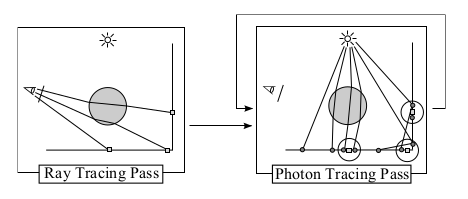
\includegraphics[width=0.7\textwidth]{overall}
\end{figure}
以下为详细算法剖分:
\subsection{Lighting Equation}
\begin{thmdef}
BRDF(双向反射分布函数), 全称为Bidirectional Reflectance Distribution Function,%
用来定义给定入射方向上的辐射照度如何影响给定出射方向上的辐射率。%
更笼统地说,它描述了入射光线经过某个表面反射后在各个出射方向上的分布效果。
\end{thmdef}\par
利用BRDF描述光照方程,即,
\begin{align}
L_o&=\int_{i\in in}BRDF(\omega_i,\omega_o)\mathop{d\!}E_i\\
&=\int_{i\in in}BRDF(\omega_i,\omega_o)L_i\cos\theta_i\mathop{d\!}\omega_i
\end{align}
其中,$E_i$为入射辐照度,$L_o,L_i$分别为出射和入射辐照率,$\theta_i$为入射光与平面法线的夹角,%
$\omega_o,\omega_i$分别为出射和入射方向。\par
考虑到计算方法,将直接光照提出,得到便于计算的光照方程,
\begin{equation}
L_o(\mathbf{x},\omega_o)=L_e(\mathbf{x},\omega_o)+\int_\Omega BRDF(\mathbf{x},\omega_i,%
\omega_o)L_i(\mathbf{x},\omega_i)(\omega_i\cdot\mathbf{n})\mathop{d\!}\omega_i
\end{equation}
其中,$L_e$为直接光照,$\mathbf{x}$为空间坐标,$\mathbf{n}$为平面法向量。
\subsection{Ray Tracing Pass}
从观察点出发,通过光线追踪来获得可见点(hitpoints),同时计算直接光照的贡献。\par
算法流程如下:\\
\begin{algorithm}[H]
\caption{Ray Tracing Pass}
\LinesNumbered
\KwIn{Camera, Lights, Width, Height, Scene}
\KwOut{Hitpoints, Pre-image}
Initialize pre-image(width,height)\;
Initialize \textit{hitpoint list}\;
\For{i in range(0,width)}{
    \For{j in range(0,height)}{
        Initialize ray with (i,j) and camera place\;
        Get the intersection of ray and scene\;
        \While{intersection is specular}{
            Determine whether it is reflected or refracted\;
            Change the direction of ray\;
            Re-get intersection\;
        }
        Accumulate direct illumination\;
        Store hitpoint\;
    }
}
Return \textit{hitpoint list} and pre-image\;
\end{algorithm}
\noindent 注:\par
在镜面较多的场景中可用反(折)射次数作为阈值强制结束Ray Tracing Pass。
\subsection{Photon Tracing Pass}
每轮Photon Tracing Pass,从光源随机方向发射一批光子,追踪每个光子的运动轨迹,%
考虑到效率,将光子能量的衰减用随机被物体表面吸收(或达到折反射阈值)来控制,%
这样每个光子的能量即为定值,折反射仅改变其颜色向量(通过BRDF计算)。\par
同时,反射、折射和吸收的概率比可用Schlick's Approximation计算,
\begin{gather}
R(\theta_i)=R_0+(1-R_0)(1-\cos\theta_i)^5\\
R_0=\left(\frac{n_1-n_2}{n_1+n_2}\right)^2
\end{gather}
其中,$n_1,n_2$为分界面折射率,$R(\theta_i)$和$1-R(\theta_i)$分别为反射、%
折射或吸收的概率。之后,折射和吸收的比率可由材质参数$Tr$确定。\par
算法流程如下:\\
\begin{algorithm}[H]
\caption{Photon Tracing Pass}
\LinesNumbered
\KwIn{Lights, Scene}
\KwOut{Photon Map}
Initialize \textit{Photon Map}\;
\For{number of photons}{
    Rand its initial direction\;
    \While{photon not absorbed and not up to limitation}{
        Get its intersection with scene\;
        Store intersection in \textit{Photon Map}\;
        \If{photon not absorbed}{
            Determine whether it is reflected or refracted\;
            Update its direction\;
        }
    }
}
Return \textit{Photon Map}\;
\end{algorithm}
\noindent 注:\par
由于直接光源已在Ray Tracing Pass计算过,故每个光子与场景的第一个交点%
不必计入photon map。
\subsection{Progressive Updation}
结束Photon Tracing Pass后,需要枚举每个hitpoint,同时统计其半径$R$内光子%
对其亮度影响。\par
此处采用\textit{photon KD-Tree}优化邻近点的搜索。\par
最后减小hitpoint半径,达到每轮增加亮度的同时,收敛到正确值。\par
记$N(\mathbf{x})$为上轮后在hitpoint $\mathbf{x}$半径$R(\mathbf{x})$内的光子数,$M(\mathbf{x})$为本次新增光子数,%
同时$\hat{N}(\mathbf{x}),\hat{R}(\mathbf{x})$分别为新累计光子数和半径,则有如下更新,
\begin{gather}
\hat{N}(\mathbf{x})=N(\mathbf{x})+\alpha M(\mathbf{x})\\
\hat{R}(\mathbf{x})=R(\mathbf{x})\sqrt{\frac{N(\mathbf{x})+\alpha M(\mathbf{x})}{N(\mathbf{x})+M(\mathbf{x})}}
\end{gather}\par
同样的,记$\tau_{N}(\mathbf{x},\omega)$和$\tau_{M}(\mathbf{x},\omega)$为%
在$\mathbf{x}$处,入射光方向为$\omega$的前光强和新增光强(未乘BRDF系数),则有
\begin{equation}
\tau_{\hat{N}}(\mathbf{x},\omega)=(\tau_N(\mathbf{x},\omega)+\tau_M(\mathbf{x},\omega))%
\frac{N(\mathbf{x})+\alpha M(\mathbf{x})}{N(\mathbf{x})+M(\mathbf{x})}
\end{equation}
其中,$\alpha\in(0,1)$是一常数。再记总发射光子数为$N_{emitted}$,$\phi$为光子光强,则最终辐照率表达式为,
\begin{align}
L(\mathbf{x},\omega)
&=\int_{2\pi}BRDF(\mathbf{x},\omega,\omega')L(\mathbf{x},\omega')%
(\mathbf{n}\cdot\omega')\mathop(d\!)\omega'\\
&\approx \frac{1}{\Delta A}\sum_{p=1}^{n}BRDF(\mathbf{x},\omega,%
\omega')\Delta\phi_p(\mathbf{x_p},\omega_p)\\
&=\frac{1}{\pi R(\mathbf{x})^2}\frac{\tau(\mathbf{x},\omega)}{N_{emitted}}
\end{align}\par
详细推导及细节见\cite{ppm}。
\section{数理计算}
除了整体性的大算法,该大作业也有一些细节上的数理计算方法也值得一提。\par
这些计算虽然底层,但由于调用次数巨大,需要进行常数优化。\par
\subsection{射线与球的求交算法}
用起点$\mathbf{s}$和向量$\mathbf{v}$表示射线$l$,用球心$\mathbf{o}$和%
半径$R$表示球$S$,设点$\mathbf{d}=\mathbf{s}+x\mathbf{v}$为线圆交点,则有:
\begin{equation}
\Vert\mathbf{s}+x\mathbf{v}-\mathbf{o}\Vert=R
\label{raysphere}
\end{equation}\par
令$\mathbf{t}=\mathbf{s}-\mathbf{o}$,并展开方程(\ref{raysphere}),有,
\begin{equation}
\Vert\mathbf{t}\Vert^2-R^2+2(\mathbf{t},\mathbf{v})x%
+\Vert\mathbf{v}\Vert^2x^2=0
\end{equation}\par
再取最小正值$x$带入,即得交点。
\begin{comment}
\listingscaption{Ray \& Sphere}
\begin{minted}{c++}
// return INF if no intersection
double intersect(const Ray &ray, const Sphere &s, Point *p, double lasthit){
    Point t = ray.bgn - s.center;
    double b = 2 * dotsProduct(t, ray.vec),
           c = t.len2() - sqr(s.radius),
           delta = sqr(b) - 4 * c;
    if (delta < EPS) return INF;  // no intersection
    delta = sqrt(delta);
    double t1 = (-b - delta) / 2,  // calculate two 
           t2 = (-b + delta) / 2,  // possible answer
           res;
    if (t1 < EPS) if (t2 < EPS) return INF;  // tangent
                     else res = t2;
       else if (t2 < EPS) res = t1;
               else res = std::min(t1, t2);
    if (res >= lasthit) return INF;  // not first intersected
    *p = ray.bgn + res * ray.vec;
    return res;
}
\end{minted}
\end{comment}
\subsection{射线与空间凸多边形的求交算法}
多边形所在平面可用任意三点表示,又考虑到精度问题,便在初始化多边形时选取%
多边形上构成三角形面积最大的三点$\mathbf{c_1},\mathbf{c_2},\mathbf{c_3}$。%
求出射线与平面的交点,再带回验证是否在凸多边形内即可。\par
用起点$\mathbf{s}$和向量$\mathbf{v}$表示射线$l$,设点$\mathbf{d}=\mathbf{s}+x%
\mathbf{v}$为射线和多边形的交点。\par
因为交点在平面上,故,
\begin{equation}
\det(\mathbf{s}+x\mathbf{v}-\mathbf{c_1},\mathbf{c_2}-\mathbf{c_1},%
\mathbf{c_3}-\mathbf{c_1})=0
\end{equation}\par
令$\mathbf{t}=\mathbf{s}-\mathbf{c_1}$,$\mathbf{c'}=\mathbf{c_2}-%
\mathbf{c_1}$,$\mathbf{c''}=\mathbf{c_3}-\mathbf{c_1}$,有
\begin{align}
\det(\mathbf{t}+x\mathbf{v},\mathbf{c'},\mathbf{c''})
=&\det(\mathbf{t},\mathbf{c'},\mathbf{c''})+x\det(\mathbf{v},%
\mathbf{c'},\mathbf{c''})\\
=&\mathbf{t}_x\times yz-\mathbf{t}_y\times xz+\mathbf{t}_z\times xy\\
&+x(\mathbf{v}_x\times yz-\mathbf{v}_y\times xz+\mathbf{v}_z\times xy)\\
=&0
\end{align}
其中,
\begin{gather}
xy=\mathbf{c'}_x\mathbf{c''}_y-\mathbf{c'}_y\mathbf{c''}_x\\
xz=\mathbf{c'}_x\mathbf{c''}_z-\mathbf{c'}_z\mathbf{c''}_x\\
yz=\mathbf{c'}_y\mathbf{c''}_z-\mathbf{c'}_z\mathbf{c''}_y
\end{gather}\par
考虑如果$\mathbf{d}$在凸多边形内,则有$\mathbf{d}$在平面上每条边的左侧,%
记平面法向量为$\mathbf{n}$,多边形逆时针点序为$\{\mathbf{p_i}\}$,则有,
\begin{align}
(\mathbf{n},(\mathbf{p_{i+1}}-\mathbf{p_i})\times(\mathbf{d}-\mathbf{p_i}))
&=\det(\mathbf{n},\mathbf{p_{i+1}}-\mathbf{p_i},\mathbf{d}-\mathbf{p_i})\\
&=\det(\mathbf{p_i},\mathbf{p_{i+1}},\mathbf{n})+\det(\mathbf{p_i}-\mathbf{p_{i+1},%
\mathbf{n},\mathbf{d}})\\
&\geqslant 0
\end{align}
\begin{comment}
\listingscaption{Ray \& Polygon}
\begin{minted}{c++}
// return INF if no intersection
double intersect(const Ray &ray, const Polygon &s, Point *p, double lasthit){
    Point ts = ray.bgn - s.pList[s.c1];
    double k = ray.vec.x * s.yz - ray.vec.y * s.xz + ray.vec.z * s.xy,
           b = ts.x * s.yz - ts.y * s.xz + ts.z * s.xy;
    if (fabs(k) < EPS) return INF;  // parallel
    double t = -b / k;
    if (t < EPS || t >= lasthit) // intersection is behind 
        return INF;              // or not first intersected
    Point ret = ray.bgn + t * ray.vec;  // intersection
    // pre-calculation
    double txy = s.normvf.x * ret.y - s.normvf.y * ret.x,
           txz = s.normvf.x * ret.z - s.normvf.z * ret.x,
           tyz = s.normvf.y * ret.z - s.normvf.z * ret.y;
    for (int i = 0; i < s.num; ++i) {
        int ni = (i + 1) % s.num;
        if (determinant(s.pList[i], s.pList[ni], s.normvf) +
            (s.pList[i].x - s.pList[ni].x) * tyz -
            (s.pList[i].y - s.pList[ni].y) * txz +
            (s.pList[i].z - s.pList[ni].z) * txy < -EPS)
            return INF;  // not on the left
    }
    *p = ret;
    return t;
}
\end{minted}
\end{comment}
\subsection{射线与KD-Tree节点立方体的判交算法}
经过尝试,传统KD-Tree在片元较多时光线判交复杂度过大,难以胜任,故我们改进了%
传统KD-Tree建法:\par
\textit{%
枚举$x,y,z$三个方向的剖分方法,选出每个方向的最优剖分面(最优被定义为完全%
在左侧的面片和完全在右侧的面片个数差尽量小),经过比较,选出最终分界面。然后%
将面片分为三组:分界面左侧,经过分界面和分界面右侧。再递归构造左子树、%
中子树与右子树。}\par
此建树方法,考虑到了经过分界面的面片数量不会太多,且左右区域的包围盒不交时,%
便于后续射线求交的剪枝。事实证明,这种建树方法,结合下面介绍的剪枝算法,%
将KD-Tree判交过程加速颇多。\par
基于这样的建树模式,介绍如下判交算法:\par
首先,KD-Tree预处理出外接立方体的边界,并记录每次划分区域的分界面。\par
不失一般性地,记$t$轴为当前KD-Tree节点分界面,为$x,y,z$轴中的某一个。%
$x_{min},x_{max}$分别为立方体在$x$轴上的边界,同理定义$y_{min},y_{max}$和%
$z_{min},z_{max}$。用起点$\mathbf{s}$和向量$\mathbf{v}$表示射线$l$,%
设点$\mathbf{d}=\mathbf{s}+x\mathbf{v}$为交点。%
计算出当前射线在立方体六个平面上的交点(事实上为三对正$x$值),如果三对$x$范围%
的交为空,则表示射线与立方体无交,退出。若有交,则可行的最小值即为射线与立方体的%
交点$\mathbf{c}$(若起点$\mathbf{s}$在立方体中,则规定$\mathbf{c}=\mathbf{s}$)。\par
考虑判断该交点的位置,若在分界面左侧,则先与KD-Tree当前节点左子树判交,%
然后将交点与$\mathbf{c}$的距离与$\mathbf{s}$到中子树的最短距离$x'$进行比较,若已短于$x'$则%
不必判中子树与右子树,直接返回,反之则再与中子树判交,再考虑右子树。%
同理可得$\mathbf{c}$在分界面右侧的情况。\par
还可以加上射线方向性的剪枝。不妨考虑$\mathbf{c}$在分界面左侧,若有%
$\mathbf{v}_t\leqslant 0$,则显然$l$不会与右子树有交。值得一提的是,此时%
$l$与左子树有交并不能保证它就是最近交点,因为左包围盒与中包围盒有交时情况较为%
复杂,如下图所示:
\begin{center}
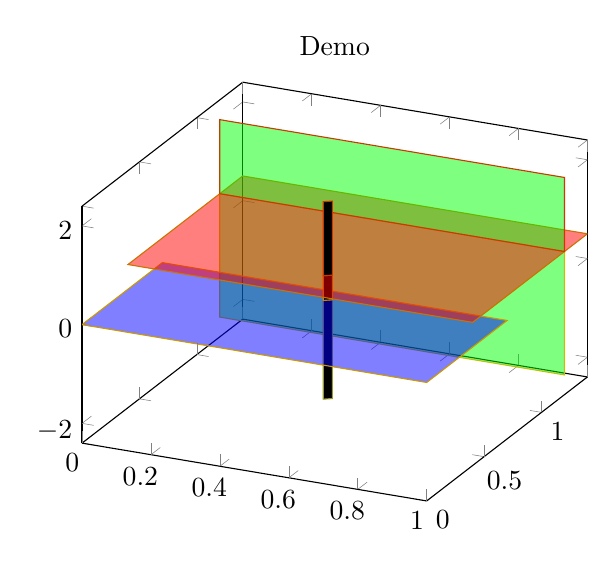
\begin{tikzpicture}
\begin{axis}[title={Demo}]
    \addplot3[surf,color={green},fill opacity=0.5] coordinates {
        (0,1.2,-2) (0,1.2,0.5)

        (1,1.2,-2) (1,1.2,0.5)
    };
    \addplot3[surf,color={black}] coordinates {
        (0.5,0.6,-2) (0.5,0.6,0)

        (0.52,0.62,-2) (0.52,0.62,0)
    };
    \addplot3[surf,color={blue},fill opacity=0.5] coordinates {
        (0,0,0) (1,0,0)
         
        (0,0.7,0) (1,0.7,0)
    };
    \addplot3[surf,color={black}] coordinates {
        (0.5,0.6,0) (0.5,0.6,0.5)

        (0.52,0.62,0) (0.52,0.62,0.5)
    };
    \addplot3[surf,color={red},fill opacity=0.5] coordinates {
        (0,0.4,0.5) (1,0.4,0.5) 
        
        (0,1.4,0.5) (1,1.4,0.5)
    };
    \addplot3[surf,color={green},fill opacity=0.5] coordinates {
        (0,1.2,0.5) (0,1.2,2)

        (1,1.2,0.5) (1,1.2,2)
    };
    \addplot3[surf,color={black}] coordinates {
        (0.5,0.6,0.5) (0.5,0.6,2)

        (0.52,0.62,0.5) (0.52,0.62,2)
    };
\end{axis}
\end{tikzpicture}
\end{center}\par
上图中绿色平面为分界面,红色面在中子树中,蓝色面在左子树中,%
黑色的射线从上而下。射线与整个包围盒的交点在左子树,故先求得射线与%
(左子树)蓝色面的交点,但是,它与中子树(红色面)的交点才是最近点。
\section{并行计算}
该算法具有高度的并行性,若能被充分利用,可很大程度上提高运行效率。
\begin{enumerate}
\item Ray Tracing Pass 中,从屏幕发出的每条光线互不相干。
\item Photon Tracing Pass 中,每个光子互不相干。
\item Progressive Updation 时,每个hitpoint互不相干。
\end{enumerate}
\section{效果展示}
\newcommand{\mygraph}[2]{
\begin{figure}[H]
  \centering
  \includegraphics[width=0.6\textwidth]{#1}
  \caption{#2}
\end{figure}
}
\mygraph{box2}{PPM原作者的场景}
\mygraph{specular}{镜面球体}
\mygraph{cyan_glass}{透明球体}
\mygraph{water}{水}
\section{总结}
\textbf{\color{red}总结有待补充}
本算法还有诸多可以提高的空间,例如:
\begin{enumerate}
\item 引入凹凸纹理贴图
\item Stochastic Progressive Photon Mapping及其他进阶算法
\end{enumerate}\par
限于时间、精力,无法进一步探索,实属遗憾。
\bibliography{Equestrotopia}
\end{document}
